\label{WG2}

\subsection{Experimental Overview}
% N. Lorenzo Martinez
 
At the time of the workshop, a number of experimental results in VBS have been made available, all of them from the LHC experiments CMS and ATLAS (see Table~\ref{tab:wg2:expres}). The highlight among these results is a measurement from the CMS experiment in the W$^\pm$W$^\pm$ channel, which for the first time shows the existence of the electroweak contribution in VBS processes at high significance (5.5 $\sigma$ observed)~\cite{CMS:2017adb}. It is interesting to notice that apart from this observation only one evidence has been found, for the VBS production in the Z$\gamma$ channel, demonstrating the experimental complexity of this process. 

\begin{table}[htb]
\centering
\begin{tabular}{|l|c|c|}
    \hline
    channel & ATLAS & CMS \\
    \hline
    $Z(\ell\ell)\gamma$ & \cite{Aaboud:2017pds} & \cite{Khachatryan:2017jub} \\
    $Z(\nu\nu)\gamma$ &  \cite{Aaboud:2017pds}& $\times$ \\
    W$^\pm$W$^\pm$ & \cite{Aaboud:2016ffv} & \cite{CMS:2017adb} \\
    W$(\ell\nu)\gamma$ & $\times$ & \cite{Khachatryan:2016vif} \\
    Z$(\ell\ell)$Z$(\ell\ell)$&  $\times$  & \cite{CMS-PAS-SMP-17-006} \\
    W$(\ell\nu)Z(\ell\ell)$ & \cite{Aad:2016ett} & $\times$ \\
    W$(\ell\nu)V(qq)$ & \cite{Aaboud:2016uuk} & $\times$ \\
    \hline
  \end{tabular}  
\caption{\label{tab:wg2:expres} Experimental results on VBS processes by final state. Only the most recent result from each experiment is shown.}
\end{table}

By now, a large fraction of the different possible final state boson combinations have been studied by at least one experiment, with the notable absence of the $\gamma\gamma$ and W$^\pm$W$^\mp$ channels, which are much more complex to reach given the amount of experimental background associated to these processes. This wide coverage of channels has been shown to be very helpful when constraining aQGCs, as the different channels show varying sensitivity to different operators, as shown in Figure~\ref{fig:EFT}.
With the larger datasets collected during the second phase of exploitation of LHC (Run2), the hope is that the experiments will be able to study the channels they did not cover yet, and be more precise on the other ones. 
%\textbf{add some figure here?} Even though, progress has been made, it would still be advantegeous if both experiments could cover all relevant channels.

\begin{figure}[h!]
    \begin{center}
    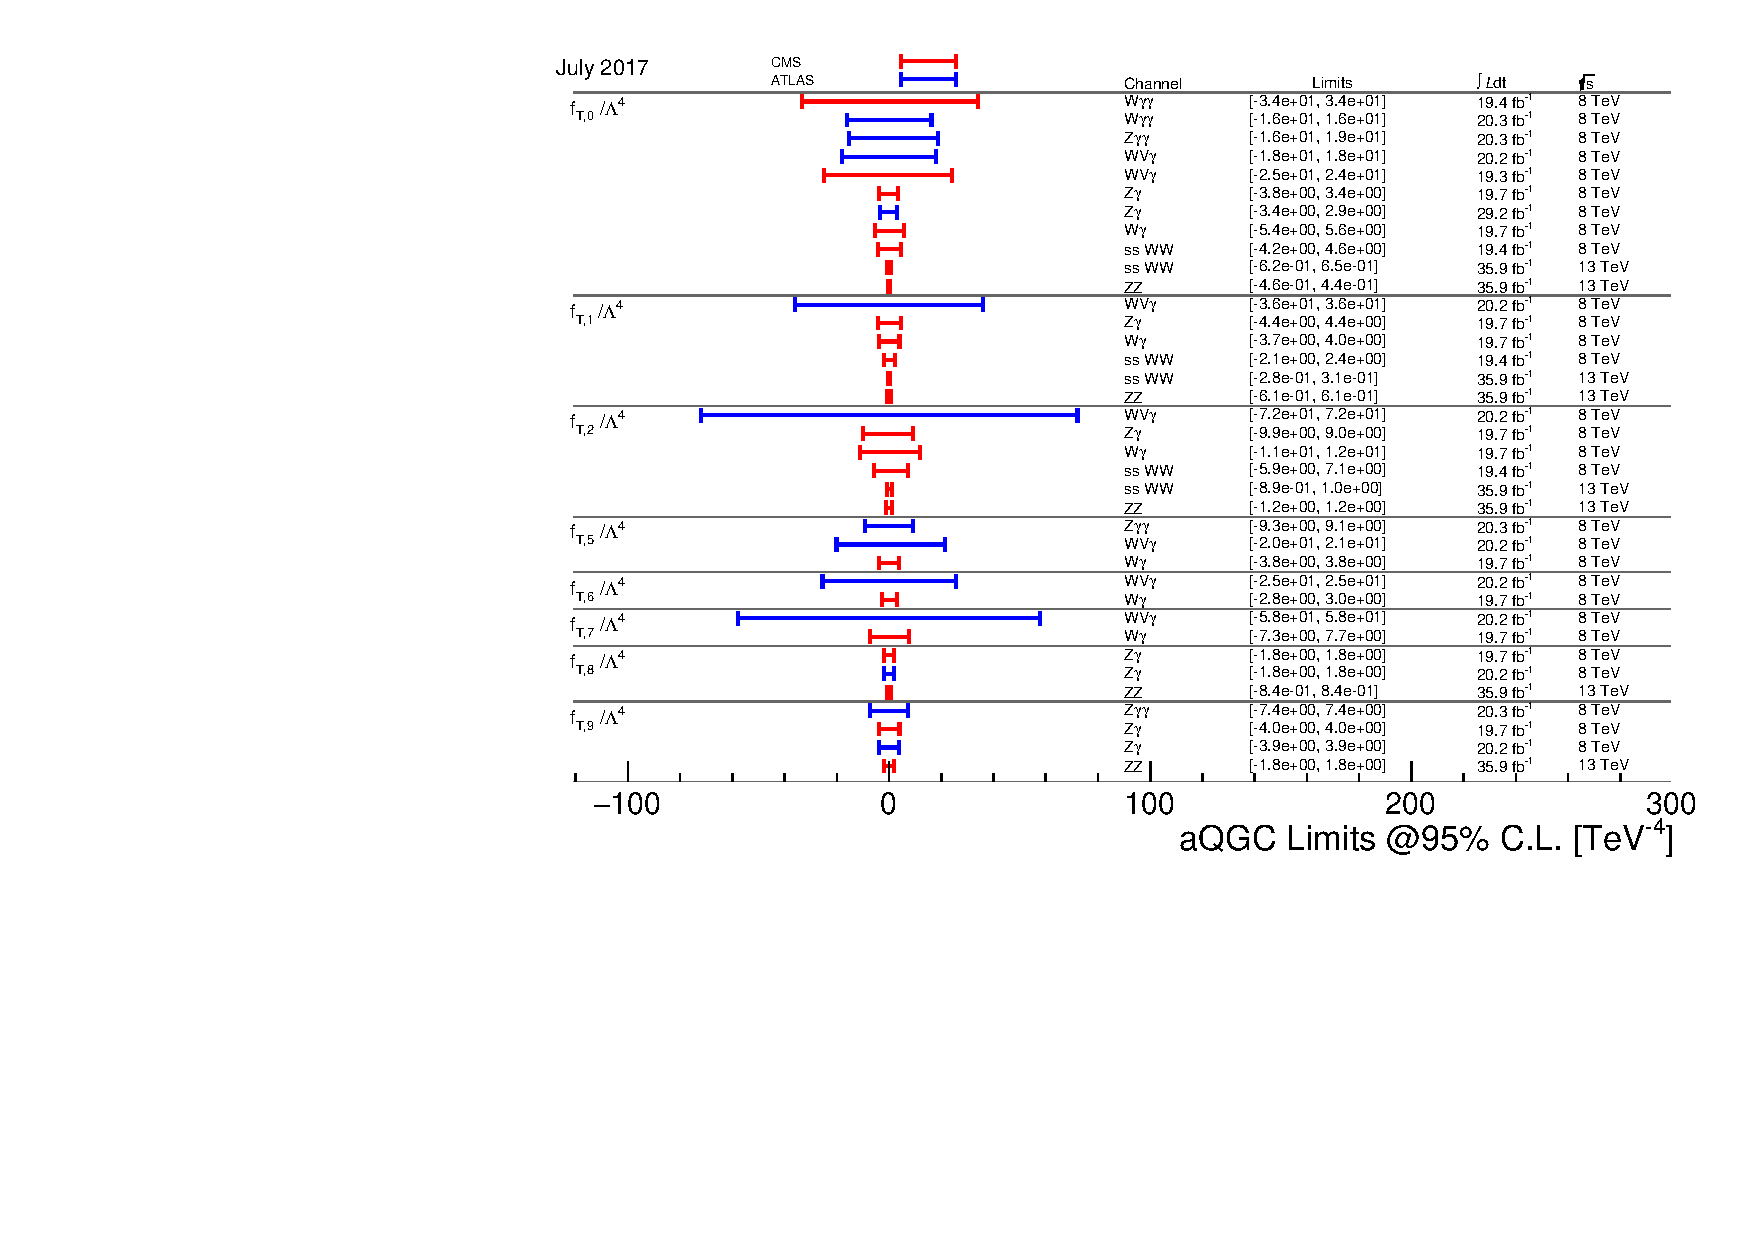
\includegraphics[width=11cm,scale=1]{figures/aQGC_ft}
    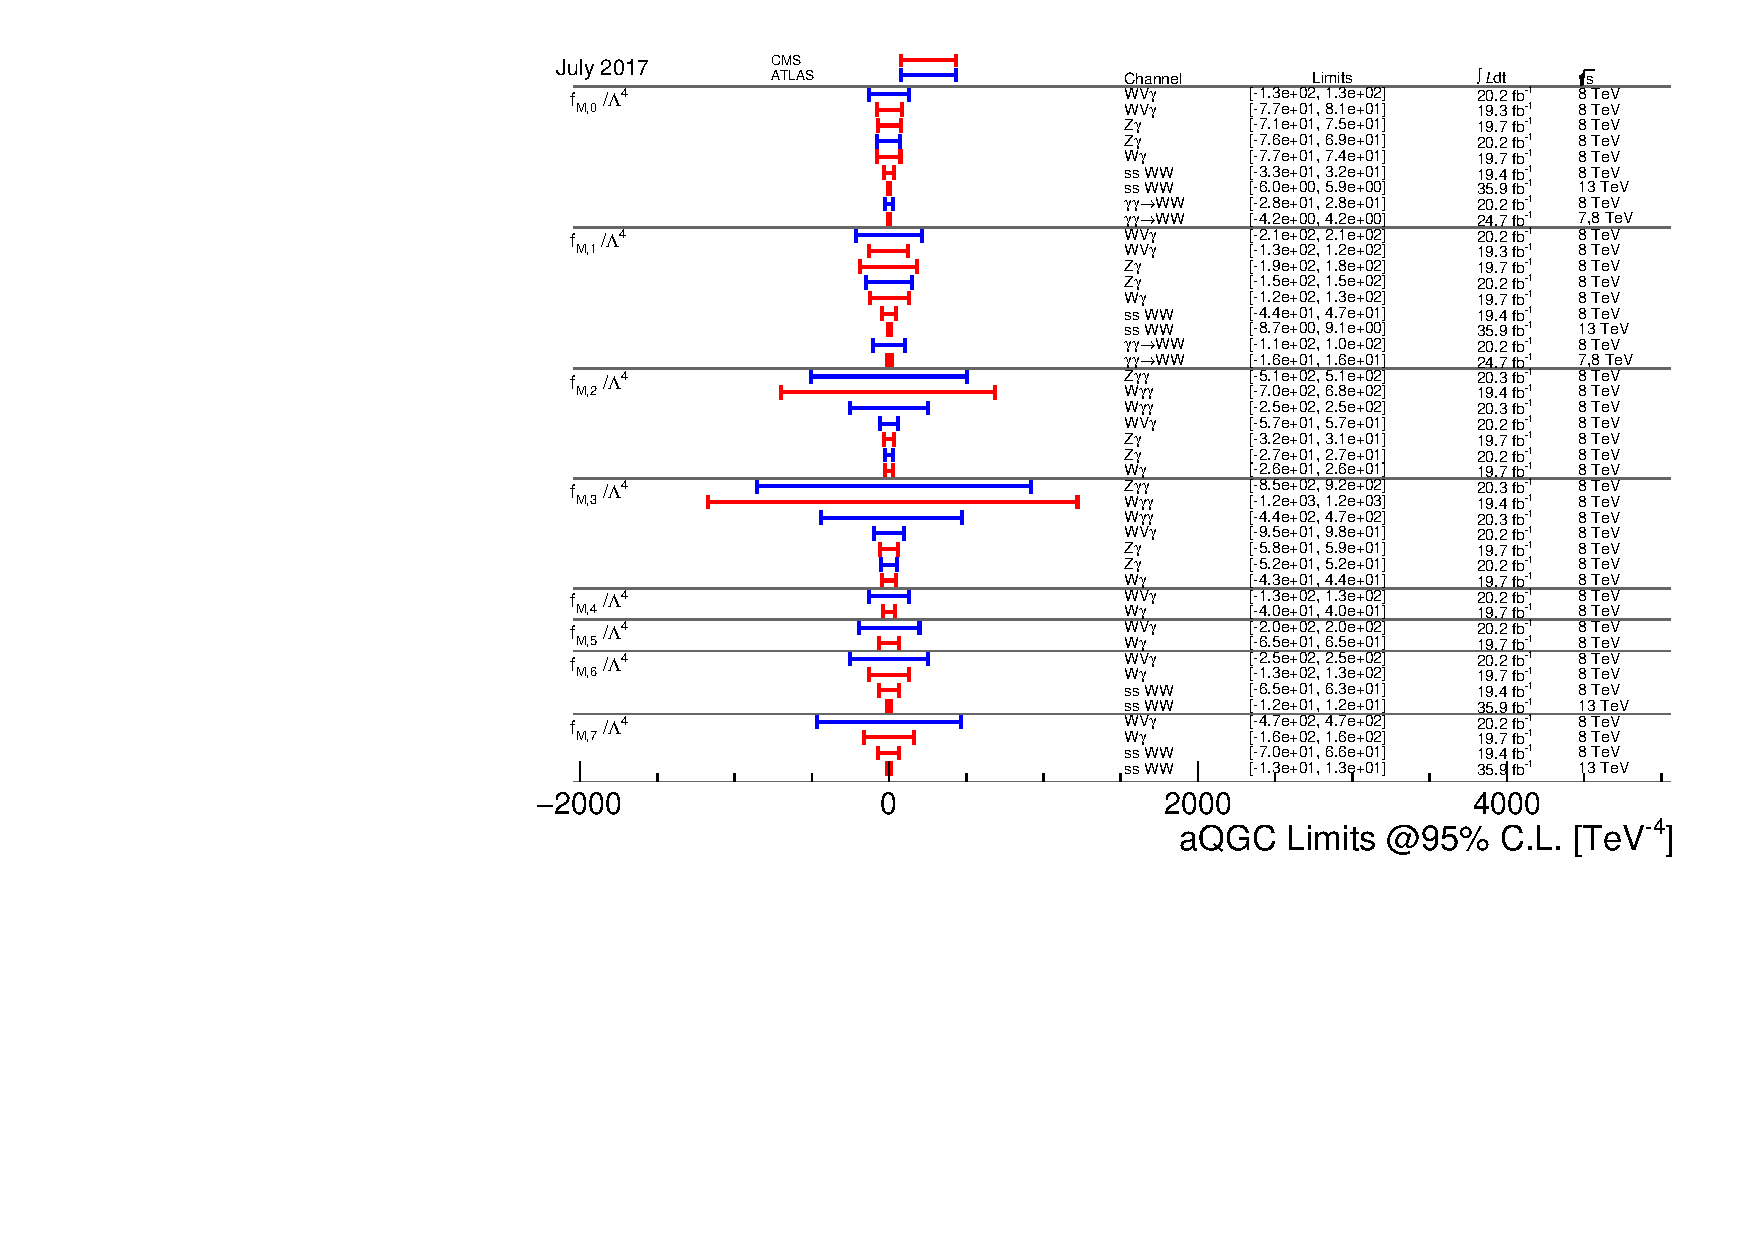
\includegraphics[width=11cm,scale=1]{figures/aQGC_fm-2}
    \end{center}
    \caption{limits on dimension 8 mixed transverse and longitudinal and transverse parameters $f_{M,i}$ and $f_{T,i}$ respectively.}
    \label{fig:EFT}
\end{figure}


%Although the avialability of such a wide range of results bodes well for future progress, the presentation and interpretation of results in the presented studies shows some notable differences.
The presentation and interpretation of results in the VBS studies reviewed during the workshop show some notable differences.

%Different approaches are used to treat unitarity issues that can arise when the analysis sensitivity to potential aQGCs is not high enough to exclude aQGC values small enough to guarnatee unitarity within the LHCs energy scale. Chosing different approaches here severly complicates the combination of different measurements of limits on aQGCs, even though such combinations could substantially increase the statistical power of the total dataset as well as break degeneracies between the effects of different operators which may affect a single channel in similar ways.

%Different approaches are chosen when treating the interference effects between electroweak and QCD amplitudes in the predictions for SM cross sections. Again, such differences complicate the combination of results, though for this effect the combination of SM cross section measurements is affected. At the current level of experimental accuracy, the differences in treatement of interference effects are still small compared to experimental accuracy, but with the continued data-taking at the LHC a common approach would be desireable. 

%Providing recommendations to resolve the above two issues should be an important goal for WG2. {\bf This doesn't sound so nice, but how to improve}

The first difference is on the treatment of interference between electroweak and QCD amplitudes in the predictions for SM cross sections. Most of the time, the interference is derived from the MadGraph~\cite{Alwall:2007fs} or Phantom~\cite{Ballestrero:2007xq} generators, and is treated as systematic uncertainty on the signal yield, leading to 5-10\% uncertainties. But in some cases, the interference is treated as a signal (ssWW ATLAS) or neglected when found to be too small (generally below 4\%). Such differences could complicate the combination of results.
%though for this effect of SM cross section measurements is affected. 
However, at the current level of experimental accuracy, the differences in treatment of interference effects are still small compared to experimental accuracy, but with the continued data-taking at the LHC a common approach would be desirable.

Another difference is the framework in which the aQGCs results are interpreted. There are mainly two approaches: one based on the C,P conserving dimension-8 EFT operators that maintains $Su(2)_L \times U(1)_Y$ gauge symmetry of the type $\phi/\lambda{}4$ (ATLAS Zg, CMS Zg, Wg, ssWW, ZZ), the other one based on the $\alpha_4$ and $\alpha_5$ coefficients of the two linearly independent dim4 operators contributing to aQGCs (ATLAS WZ, ssWW, WV semilept). Even if the conversion between the two frameworks can be done, it can be better for quick comparison and combination to adopt an unique framework.

Finally, another difference lies in the treatment of unitarity issues that can arise when the analysis sensitivity to potential aQGCs is not high enough to exclude aQGC values small enough to guarantee unitarity within the LHC energy scale. In the $\alpha_4$, $\alpha_5$ framework, the unitarisation is done with the so-called K-matrix method, within the WHIZARD generator. In the dimension-8 EFT operator framework, two approaches are used by ATLAS and CMS, respectively. ATLAS uses a form factor of the type $f_i/(1+s/\Lambda_{FF^2})^n$, where $n=2$ and $\Lambda_{FF}$ is the cut-off scale. CMS, on its side, only provides a validity bound, i.e the scattering energy at which the observed limit would violate the unitarity, derived from the VBFNLO generator. Some of the results published by the collaboration show that at the LHC scales, already many limits are set in the unitarity unsafe region. 
Choosing different approaches could severely complicate the combination of different aQGCs limits measurements. Performing such combinations could substantially increase the statistical power of the total dataset and could help to break degeneracies between the effects of different operators which may affect a single channel in similar ways.

Providing recommendations to unify the treatments mentioned above is an important goal for WG2. 

Another lesson learned from the experimental review was the modeling issue affecting the main background producing the same final state via QCD interactions. To mitigate this effect, experiments use control regions (generally low dijet invariant mass) in which they constrain and verify the QCD background normalization and shape. While until now the precision is not enough to constrain these quantities, with more statistics it will become more relevant and QCD modeling issues could be a limiting factor in the analyses.

The measurements are currently dominated by the uncertainty on the jet energy scale and resolution, and by background estimation and theory uncertainties (scales, pdf). This together with the previous point will be important to mitigate in the future: this is one of the goals of WG2 and WG3.
 
Finally, it is interesting to notice the importance of the constraining power of the WV channel, where V is a W or Z boson decaying hadronically. Thanks to advanced jet substructure techniques, this channel brings the tightest constraint on EFT charged parameters, since its boosted topology allows to reach higher energy regimes. This will be also a goal of WG3 to continue developing such techniques. 
\subsection{Common Selection Criteria}
% X. Janssen

In order to facilitate feasibility studies and similar forward looking analysis in a way that allows for a fair comparison between such studies, it will be useful to define a common baseline for a fiducial phase space. However, a single definition cannot serve as the base for every study for the following reasons:
\begin{itemize}
\item The experiments themselves will evolve due to hardware upgrades planned for the high luminosity phase of the LHC, necessitating different assumptions on the detector acceptance depending on the integrated luminosity used for the forward lookgin study.
\item Different final VBS channels and different boson decay modes may require notably different selection criteria.
\end{itemize}

The simplest case is realized for near term studies of VBS channels with signals large enough to be amenable to a simple ``cut \& count'' style analysis, notably the W$^\pm$W$^\pm$ channel. Based on published results, a phase-space region close to CMS as well as ATLAS studies has been identified (see Table~\ref{tab:wg2:phasespace}). This is likely to be useful for forward looking studies reaching up to, but excluding the high luminosity phase of the LHC.

Further extrapolation into the future suffers from the problem, that the design work for the envisioned detector upgrades is not entirely completed yet, so that work in this area is necessarily somewhat speculative. Nevertheless a few general conclusions can be drawn from existing detector design documents. Both experiments plan to improve their trigger systems to keep the thresholds for lepton triggers at a similar level to current running conditions, so that $p_{\mathrm{T}}$ thresholds should remain close to current ones. Both experiments also plan to extend coverage of their respective tracking detectors up to $|\eta|\sim 4$. However due to differences in the other systems relevant for lepton identification (electromagnetic calorimeter and muons systems), the final geometric coverage for the leptons is not yet certain and may differ substantially between experiments.

While the common phase space definitions discussed here are useful for the study of channels that are experimentally accessible with straight forward techniques, they are less suitable for studies of channels with very low cross section, branching fraction or efficiency, as exemplified by the ZZ$\rightarrow 4\ell$ channel. Due to the low number of observable events in this channel, the existing analysis~\cite{CMS-PAS-SMP-17-006} is performed in a very inclusive phase space, employing sophisticated mutli-variate techniques to isolate the signal. Such multivariate techniques are difficult to model in forward looking studies in a simple manner, and an ad-hoc implementation of a  ``cut \& count'' style study is likely to severally underestimate the future performance of the LHC detectors. For this case, the scaling of existing results according to the expected growth with luminosity of signal and background yields, will be preferable.

\begin{table}[htb]
\centering
\begin{tabular}{|l|l|l|l|l|}
    \hline
             & electrons & muons & jets & photons \\
    \hline
    $|\eta|$ & $<2.5$  & $<2.4$ & $<4.5$ & $<2.5$ \\
    $p_\mathrm{T,lead.}$ & $>25$~GeV & $>25$~GeV &$>30$~GeV &$>25$~GeV\\
    $p_\mathrm{T,sublead.}$ & $>15$~GeV & $>15$~GeV &&\\                            
    \hline
  \end{tabular}  

\caption{\label{tab:wg2:phasespace} Proposed phase space for studies in the WW channel.}
\end{table}

\subsection{Prospects}
% M. Kobel

The presentation touched on several major topics interesting for future studies. First among these was the study of the final state bosons polarisation fractions. The scattering of longitudinal vector bosons violates unitarity in the absence of a standard model Higgs boson. By looking at the scattering of electroweak gauge bosons we will be probing the Higgs properties. %Such a measurement would allow for the isolation of the scattering component of longitudinally polarised bosons, which is of particular interest due to its connection to the Higgs sector.
The polarisation is accessible through the angular distributions of the boson decay products in the boson rest frame. 
Measurements of the polarisation for VBS are particularly challenging because in the cleanest channel ($W^\pm W^\pm$), the decay products include two neutrinos, which prevent a straight-forward reconstruction of the boson decay angular distribution. Other channels, which allow for the reconstruction of these angular distributions, on the other hand, suffer from much larger backgrounds. Several potential approaches to address this issues were presented, including a number of mass-like variables, which extract polarisation information even from final states with two neutrinos as well as a study using neural networks. 

%\begin{figure}[!h] 
%\begin{centering}
%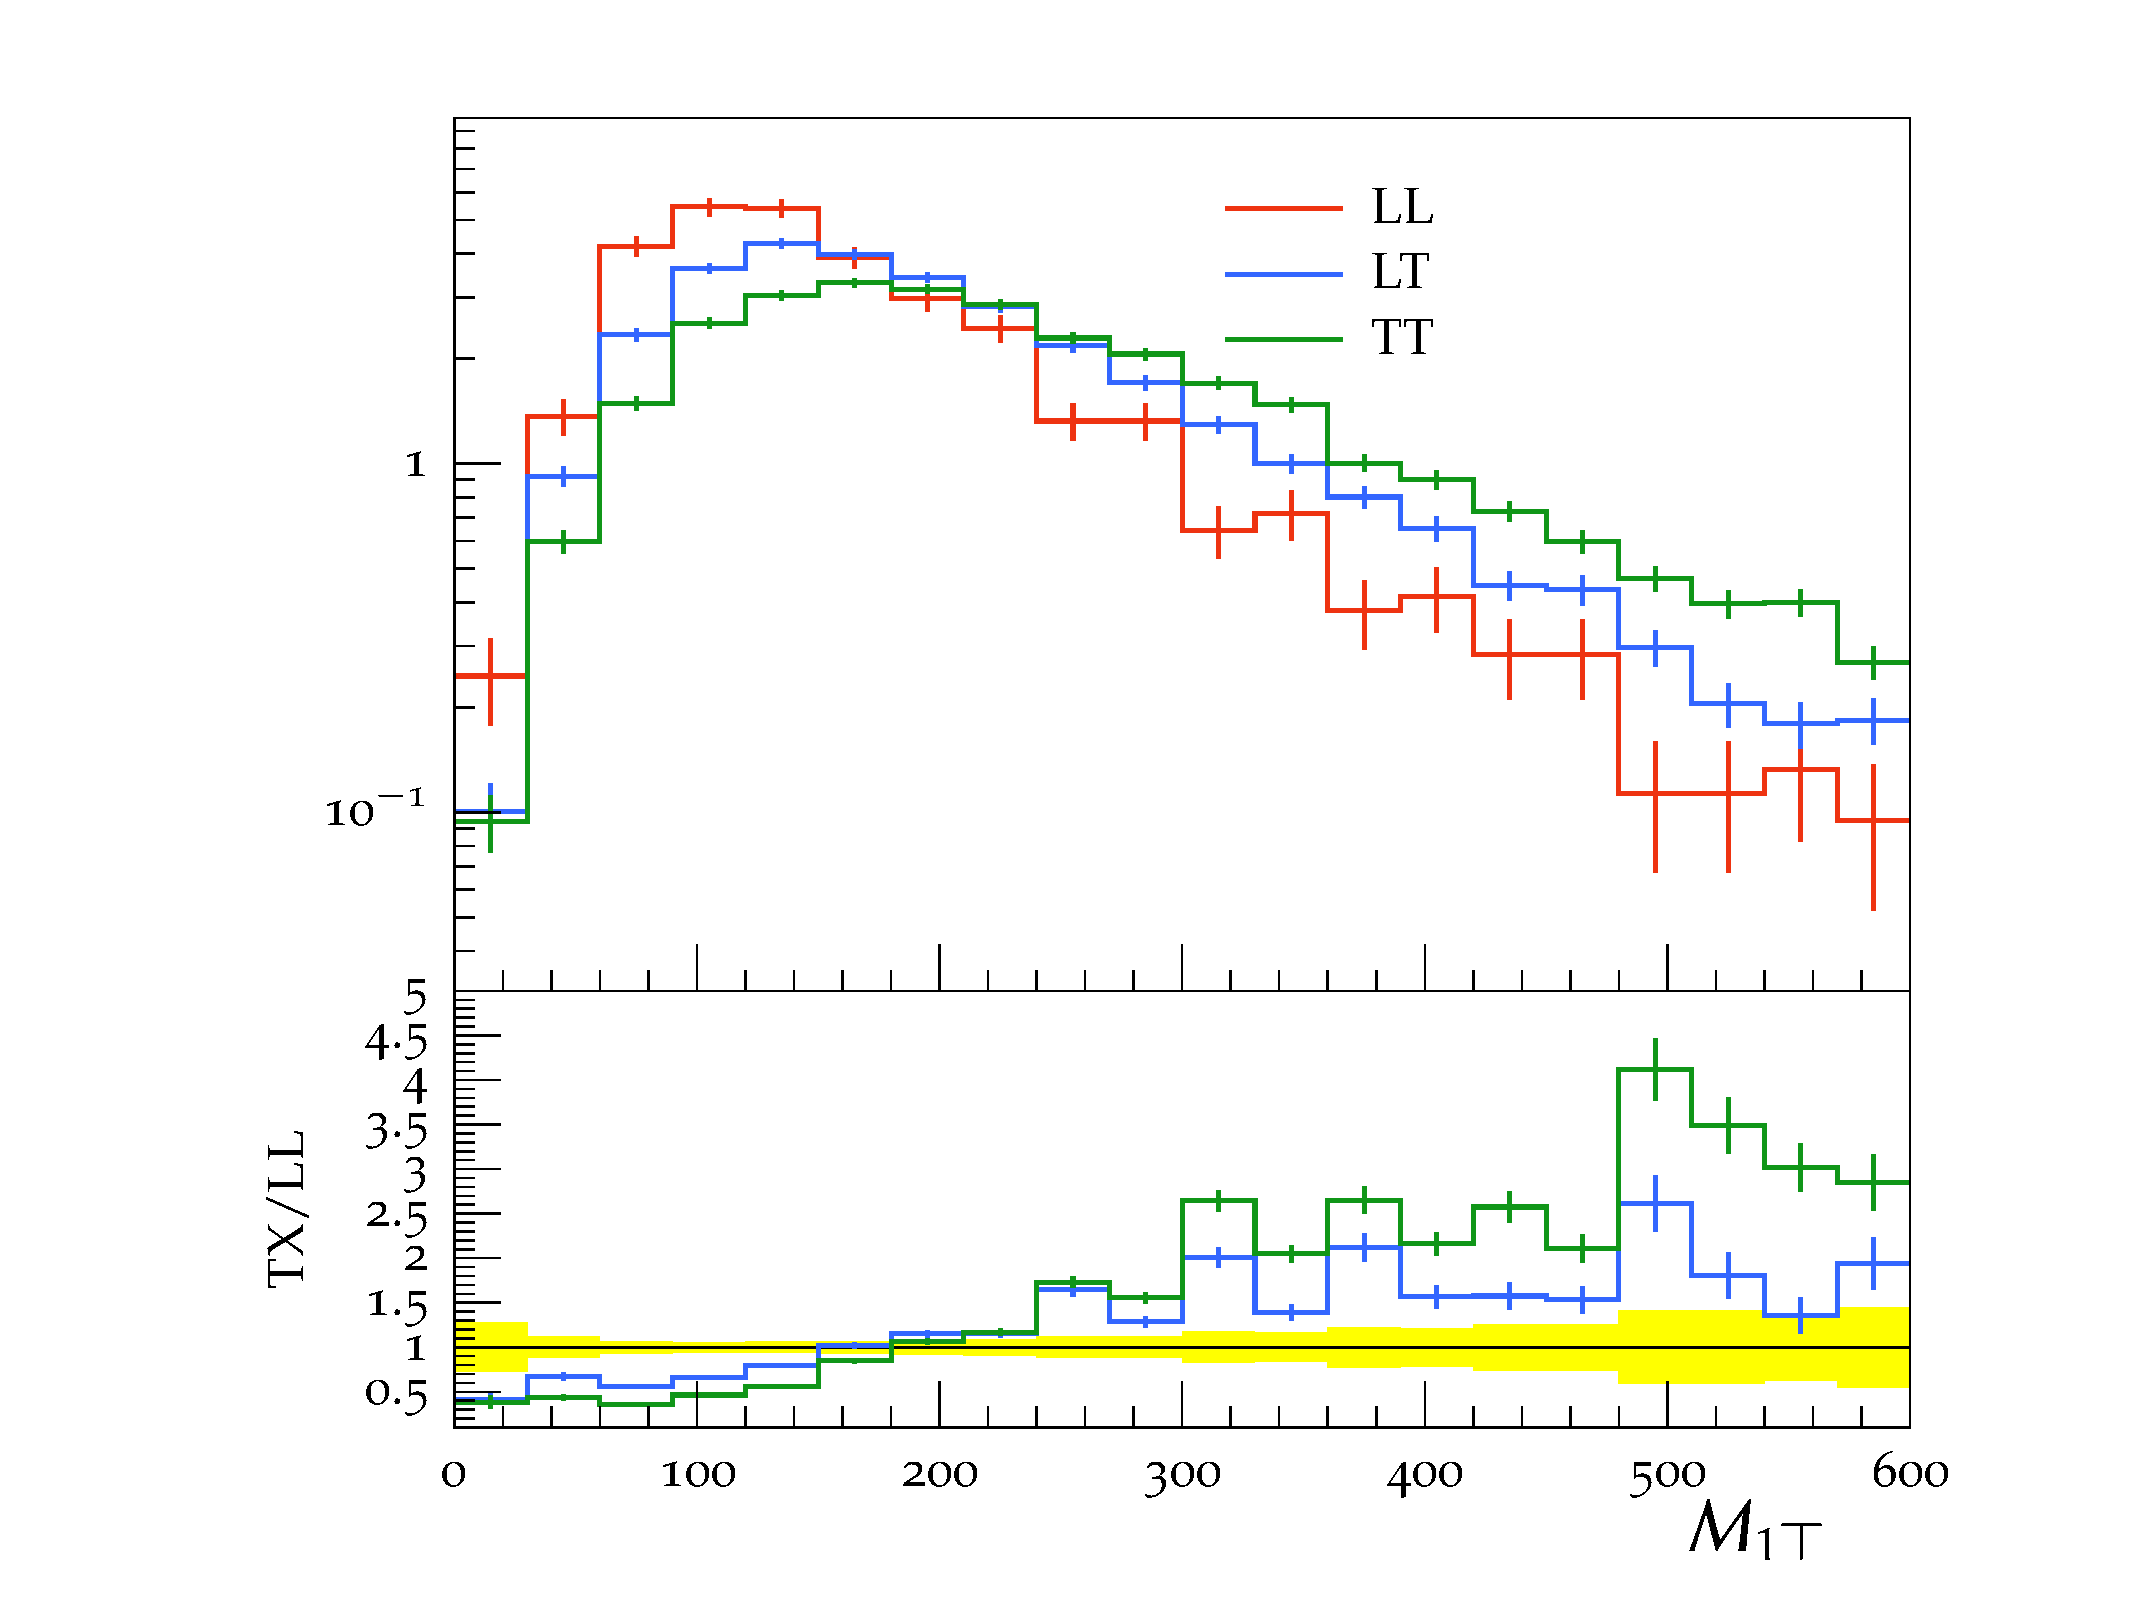
\includegraphics[width=0.48\textwidth]{WG2_plots/M1T.pdf}
%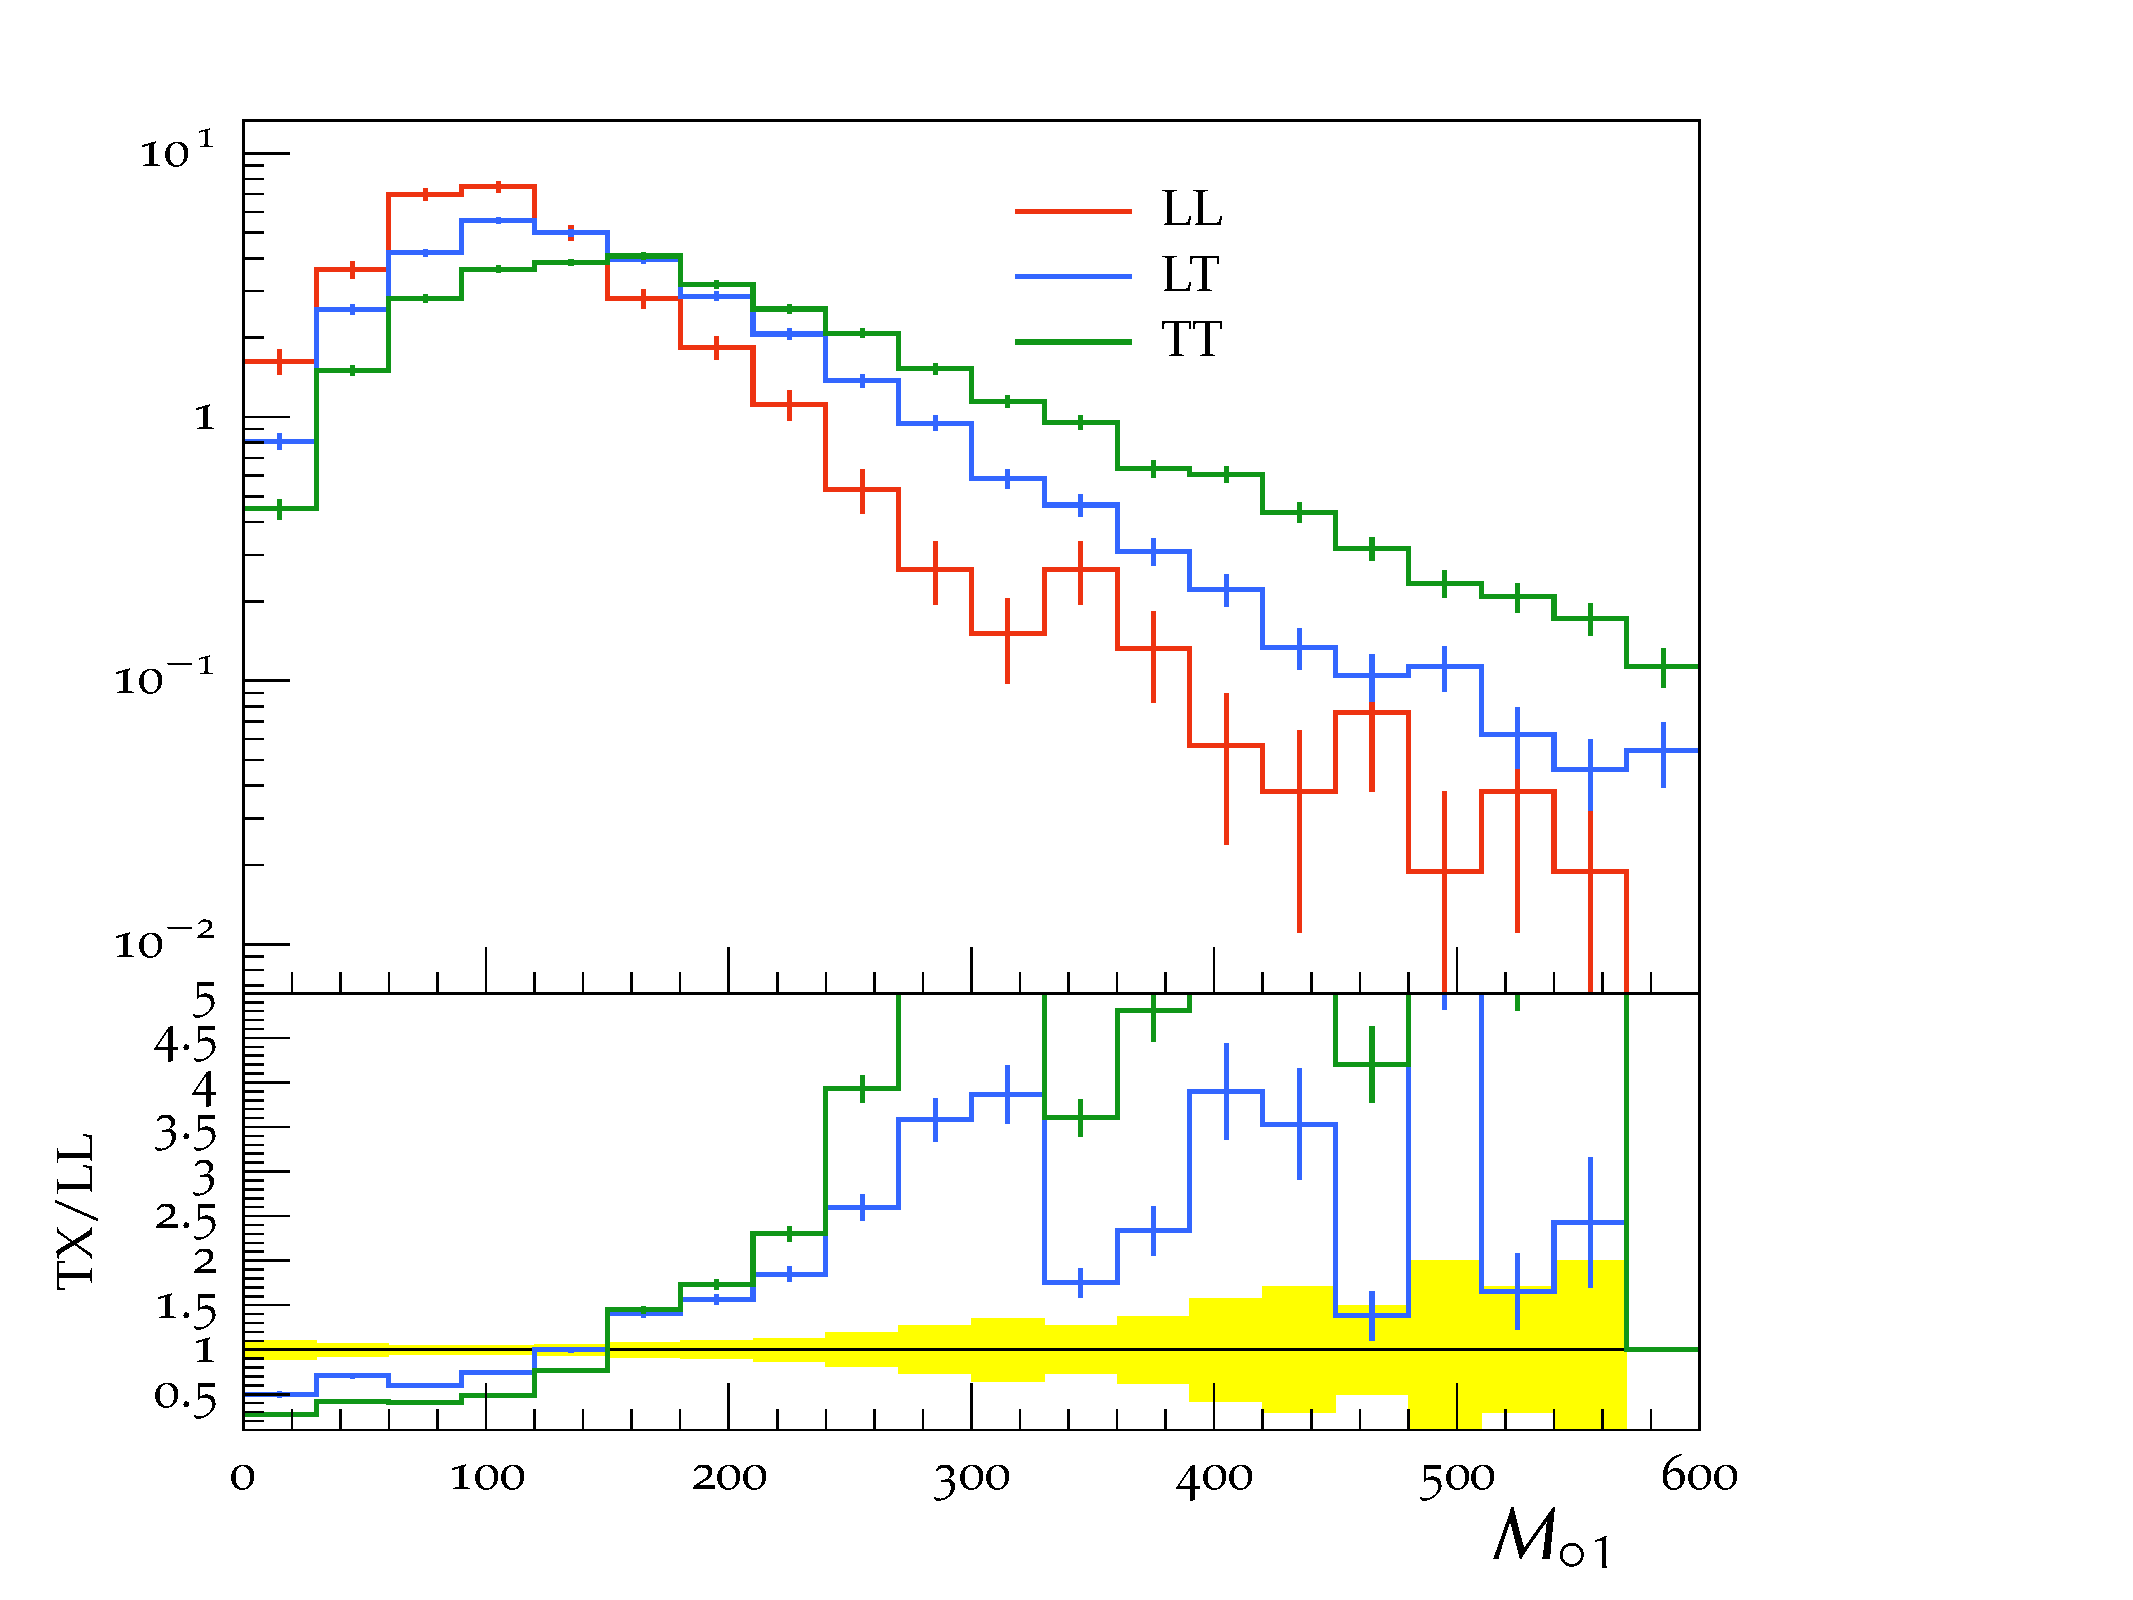
\includegraphics[width=0.48\textwidth]{WG2_plots/Mo1.pdf}
%\caption{}
%\label{fig:massWW}
%\end{centering}
%\end{figure}

As a topic for future studies, the presentation discussed potential information to be gained by measuring the relative cross sections of different VBS channels, in particular channels related by charge symmetry. Beyond the naive expectations related to the valence quark content of the proton, it can be shown that these ratios can provide sensitivity to BSM processes, but also provide constraints on the effects of the underlying parton density functions, which may otherwise be erroneously be interpreted as deviations from the SM.

Additionally, the interpretation of experimental results in terms of BSM effects was discussed. While the EFT approach discussed above has the advantage of being generic and provides a complete description of a very wide range of BSM models, there is also a number of shortcomings. However, anomalous couplings of a size that will cause observable effects at low scales, will  commonly violate unitarity at high scales, so that ad-hoc approaches to unitarization are applied which introduce a new model-dependence: the dependence on the unitarization scheme.
Beyond this, there is the issue that the EFT is only valid in the approximation that the scale of the observed scattering is much smaller than the scale $\Lambda$. Empirical studies, comparing explicit resonance models to EFTs, show that the \textit{amount} by which the $\Lambda$ has to exceed the described region of data can be substantial, to the point where visible effects that are accurately described by an EFT would correspond to theories so strongly coupled, that their treatment in perturbation theory would be questionable. A way to avoid these problems would be an interpretation using a simplified resonance parameterization, which does not run into unitarity issues, but is by construction less general than the EFT approach.



